This section provides detailed information about the system with its components.


\subsubsection{System Perspective}
OpenFlexure is not a part of a larger system. However, it interacts OpenFlexure Development Server in order to keep the system software up-to-date. Additionally, the communication between the OpenFlexure and Users is provided by OpenFlexure Web API. Users will be able to send their requests using the Web API and get responds from the server again using this API.

There are three user types in the system: User (can be seen as end-user), Admin and Maintainer. The system will provide different interfaces to each of them so that they can do the functions defined to them. Since admins and maintainers have private permissions, they will need to log in to the system using the keys defined to them in order to use their functions. While Admins and maintainers will be responsible for keeping the system stable, Users will be able to control and use OpenFlexure Microscope.

\begin{figure}[H]
	\centering
	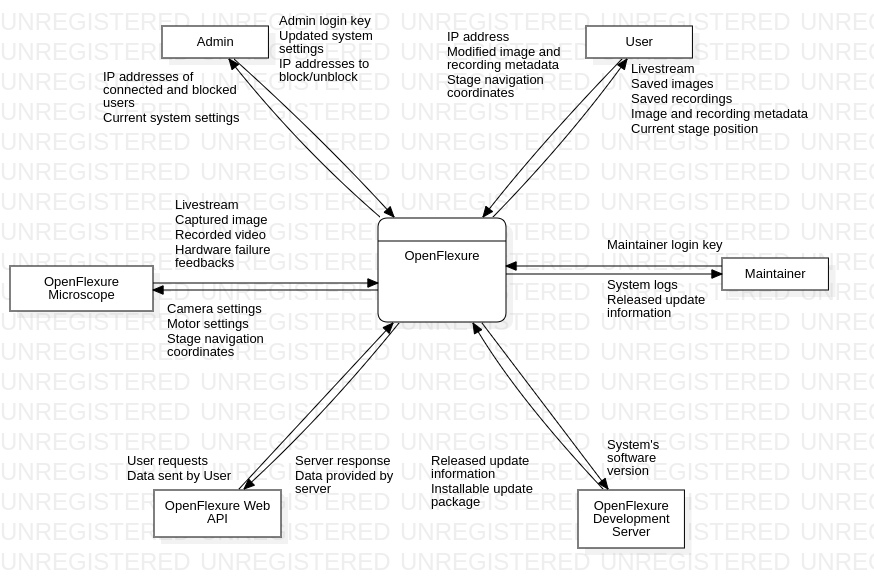
\includegraphics[scale=0.5]{Uml_Images/system_context_diagram}
	\caption{System Context Diagram for OpenFlexure}
	\label{fig:system_context_diagram}
\end{figure}


\paragraph{System Interfaces} 
\subparagraph{Database Management Interface: } Database Management Interface is one of the primary components of OpenFlexure. It allows storing the IP addresses of users, activities of users, login keys of administrators and maintainers, error logs, etc. When any other interface wants to write to or read from the database, Database Management Interface provides a stable and secure connection to the system database.
\subparagraph{Back-end Failure Management Interface: } Due to the nature of the microscope components, it is highly possible to have hardware and software failures in microscopes. Managing these failures and acknowledging the responsible staff (maintainers) is a crucial task. This interface is always active in case of handle any system failures. It is responsible for detecting anomalies and failures in the system and keeping detailed logs about the situations. When the interface detects a failure, it communicates with the Database Management Interface to store the error logs in a protected database area that can be reached by maintainers.


\paragraph{User Interfaces}
\subparagraph{User Connection Interface:} OpenFlexure desktop application will provide connection interface to the users. Desktop application is not mandatory to connect the system. If user is already know the ip address of the microscope, he/she can directly open User Web Interface by entering the ip address from his/her browser. Desktop application is helpful to detect the microscope servers nearby the user.
\subparagraph{User Web Interface:} User will be able to control microscope and view the camera feed using the user web interface. Web interface will provide live stream camera feed, navigation menu to change the position of the stage and gallery window to view saved media. User will be able to reach to User Web Interface by just typing the ip address of the microscope's server. The GUI will send the events to Web API, then Web API will transform these events to HTTPS requests. 
\begin{figure}[H]
	\centering
	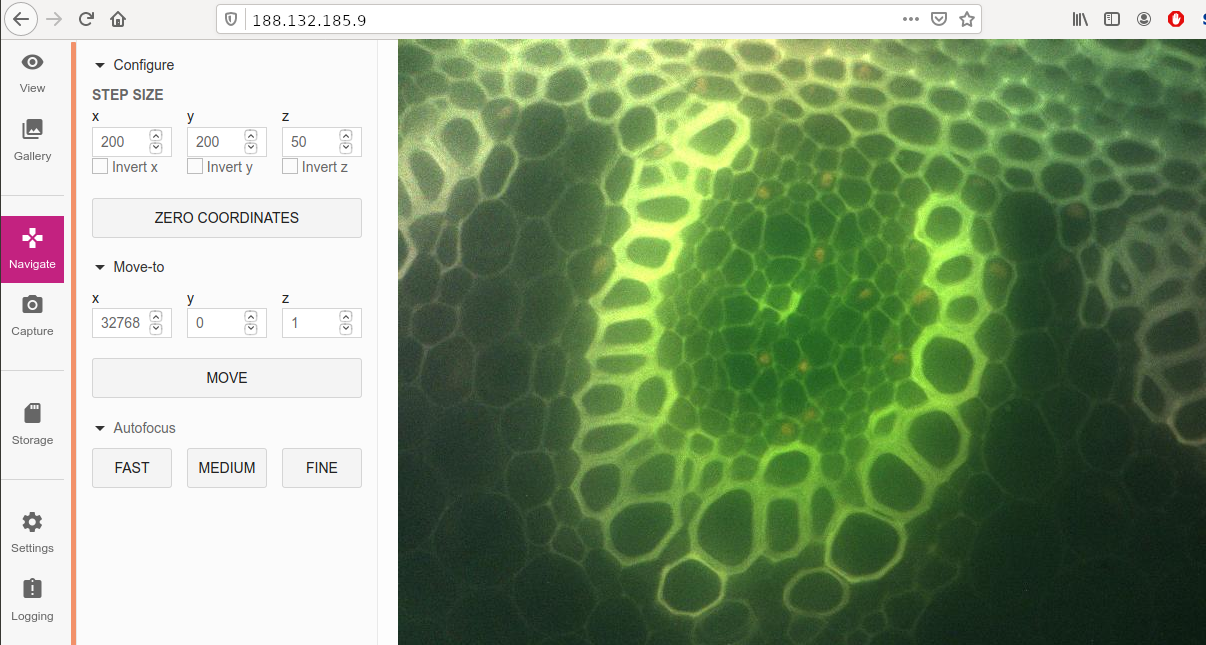
\includegraphics[scale=0.3]{Figures/user_web_interface}
	\caption{OpenFlexure User Web Interface}
	\label{fig:user_web_interface}
\end{figure}
\subparagraph{System Admin Management Interface:} System administrators will use a command-line interface to manage the system. The reason to use a command-line interface rather than GUI is related to speed. Administrators should be able to apply their actions immediately. Since the command-line interface is a more quick way to apply actions, it is preferred over GUI. Administrators will be able to list the detailed information about connected/blocked users and system settings. Using the commands provided by this interface, the administrators will be able to manage/update system settings and block/unblock users.
\begin{figure}[H]
	\centering
	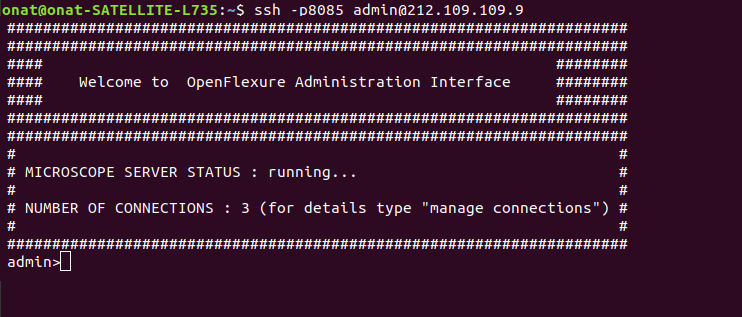
\includegraphics[scale=0.5]{Figures/admin_interface}
	\caption{OpenFlexure Administration Command-line Interface}
	\label{fig:system_admin_management_interface}
\end{figure}
\subparagraph{Maintainer Management Interface:} Similar to system administrators, the maintainers will also use a command-line interface to manage the system, due to the similar reasons. Since the permissions of the maintainers are limited to system update and retrieving the system logs, commands available to maintainers will also be limited. Maintainer will be able to list saved error logs, system details such as software versions and the information about the latest software updates. Furthermore, maintainers will be able to update the system softwares using the command provided by this interface.

\paragraph{Software Interfaces}
\begin{itemize}
	\item Python 3.8 is used for back-end operations
	\item Flask 1.1.2 is used to implement web application
	\item PostgreSQL 13.2 is used as database management system
\end{itemize}

\paragraph{Communications Interfaces}\mbox{}\\
Desktop application and web application uses HTTPS protocol to communicate with the back-end system.

\paragraph{Hardware Interfaces}\mbox{}\\
OpenFlexure microscopes have two main hardware components: Raspberry Pi camera system to retrieve the livestream, captured image-video data, and motor system to control the position of the stage. To manage and communicate with these components, the system shall have two hardware interfaces:
\subparagraph{Camera System Interface:} The Camera System Interface is a medium between a Raspberry Pi Camera and the server. The server retrieves the livestream and captured image-video data using the Camera System Interface. Additionally, camera configurations such as frame rate, resolution, and commands such as capture image, record video are also transferred to the Raspberry Pi Camera using this interface.
\subparagraph{Motor System Interface:} The microscope shall have three motors to control the stage in the x, y, and z axes. These motors will be controlled by an Arduino Motor Controller. Motor System Interface provides a stable connection between the server and the Arduino Motor Controller. The system gives the navigation coordinates of the stage to Arduino Motor Controller using this interface.\\

Both the Camera System Interface and Motor System Interface also communicate with the Back-end Failure Management Interface to report any hardware-related failures.

\paragraph{Memory Constraints}\mbox{}\\
System engineering is already handled for the OpenFlexure Microscope system as a whole.
\paragraph{Operations}\mbox{}\\
The operations of the OpenFlexure system can be represented as: \\
\textbf{User:}
\begin{enumerate}
	\item  Connect to Microscope
	\item  View Livestream
	\item  Record Video
	\item  Capture Image
	\item  Scan
	\item  Navigate Stage
	\item  Open Gallery
	\item  Modify Media
\end{enumerate}

\textbf{Admin:}
\begin{enumerate}
	\item  Log in as Admin
	\item Manage System Settings
	\item Manage Connections
	\item Block User
	\item Unblock User
\end{enumerate}

\textbf{Maintainer:}
\begin{enumerate}
	\item  Log in as Maintainer
	\item  View System Logs
	\item  Check Updates
	\item  Update Software
\end{enumerate}


\subsubsection{System Functions}
\begin{table}[H]
	\centering
	\begin{tabular}{|l|C|}
		\hline
		\textbf{Function}   &  \textbf{Summary}\\
		\hline
		\textbf{Connect to Microscope}   &  The user connects to the microscope's server\\
		\hline
		\textbf{View Livestream}   &  The user views the live camera feed\\
		\hline
		\textbf{Record Video}   &  The user starts recording the livestream\\
		\hline
		\textbf{Capture Image}   &  The user captures the image on the screen\\
		\hline
		\textbf{Scan}   &  The system generates a scan of the area bounded by the coordinates provided by the user\\
		\hline
		\textbf{Navigate Stage}   &  The user adjusts the position of the stage\\
		\hline
		\textbf{Open Gallery}   &  The user displays the saved images and recorded videos\\
		\hline
		\textbf{Modify Media}   &  The user modifies the saved media\\
		\hline
		\textbf{Log in as Admin}   &  The admin connects to server with his/her login key\\
		\hline
		\textbf{Manage System Settings}   &  The admin manages and updates the system settings\\
		\hline
		\textbf{Manage Connections}   &  The admin views the list of connected and blocked users\\
		\hline
		\textbf{Block User}   &  The admin blocks a user with given IP address\\
		\hline
		\textbf{Unblock User}   &  The admin unblocks a user with given IP address\\
		\hline
		\textbf{Log in as Maintainer}   &  The maintainer connects to server with his/her login key\\
		\hline
		\textbf{View System Logs}   &  The maintainer can list and view the system logs sorted by their dates\\
		\hline
		\textbf{Check Updates}   &  The maintainer checks for the software updates\\
		\hline
		\textbf{Update Software}   & The maintainer updates the system software \\
		\hline
	\end{tabular}
	\caption{System Functions}
	\label{tab:system_functions}
\end{table}


\subsubsection{User Characteristics}
The users of the OpenFlexure can be classified under three categories: users (end-users), system admins, and maintainers.
\subparagraph{Users (End-users):} are the people who connect to microscopes for regular purposes such as viewing livestream, capturing images etc. They are not authorized, and their permissions are limited. They do not need to have technical skills to use the system. In educational applications, they can be students.
\subparagraph{Admins:} are authorized people who have permission to manage connected users and manage system-wide settings. They connect to the microscope server with their private keys and use "Admin Command-line Interface" to manage the system. They are managers rather than technical staff; therefore, system configurations and operations that require technical skills are in the scope of maintainers rather than admins. Although they do not need to have advanced technical skills, they need to know how to use ssh connection and command-line interface. In educational applications, they can be lab assistants or teachers.
\subparagraph{Maintainers:} are authorized people who have permission to view system logs such as crash reports and suspicious login attempts. They are also responsible for maintaining system hardware and updating the software used. They connect to the microscope server with their private keys and use "Maintainer Command-line Interface" to handle technical operations. Maintainers are expected to have good technical skills and knowledge. In educational applications, they can be IT staff of the universities/high schools.


\subsubsection{Limitations}
\begin{itemize}
	\item \textbf{Regulatory Policies:} The system holds user IP addresses and media captured by them. Ownerships of these media belong to the users saved them. Additionally, maintainer and admin keys are also stored in the system. These data shouldn't be leaked and should be preserved encrypted.
	\item \textbf{Hardware Limitations:} The servers that process the livestream camera feed should be powerful enough to handle that. For users, internet connected computer is enough to use the system.
	\item \textbf{Interfaces to other applications:} The system should be  compatible with the OpenFlexure Development Server to install software updates. Additionally, system should be compatible with camera and motor module drivers to communicate with them.
	\item \textbf{Parallel Operation:} The system should allow multiple users to use the system at the same time. Furthermore, users should be able to perform additional operations while performing long-running operations such as tile scan. Hence, it should allow multiple threads running at the same time.
	\item \textbf{Audit Functions:} System should generate logs when any failures or suspicious login attempts happen. It is maintainers' responsibility to control these logs and fix the system.
	\item \textbf{Control Functions:} Control functions should be reachable for only maintainers and admins, and it requires necessary key verifications. Additionally, permissions of maintainers and admins are separate and maintainers cannot access admin control functions.
	\item \textbf{Higher-order  Language  Requirements:} Bash will be used for Command-line Interface, Python will be use for server-side applications since Flask is used as a web application framework.
	\item \textbf{Signal Handshake Protocols:} System should use HTTPS protocol to retrieve the requests from users and respond to them.
	\item \textbf{Quality Requirements:} Since system stores captured images and recorded videos, it is important to take backups regularly.
	\item \textbf{Criticality of the application:} Failures may cause research and education practices to be interrupted. Therefore, any system failure shall be solved quickly.
	\item \textbf{Safety and security considerations:} User database records do not contain personal information other than IP addresses. Maintainer and admin keys shall be stored in a protected database and suspicious login attempts shall be investigated by maintainers.
	\item \textbf{Physical/Mental  considerations:}	Visually and mentally impaired people may find it difficult to use the system.
\end{itemize}